\secspace
\section{Introduction}
\label{sec:intro}

It is not an exaggeration to say that the arrival of text-to-image generator
models has transformed, perhaps upended, the art industry. By sending simple
text prompts like ``A picture of a corgi on the moon'' to diffusion models
such as StableDiffusion or MidJourney, anyone can generate incredibly
detailed, high resolution artwork that previously required many hours of work
by professional artists. AI-art such as those in Figure~\ref{fig:aiart} have
won awards at established art conventions~\cite{winaward}, served as
cover images for magazines~\cite{c-ai-cover}, and used to
illustrate children's books~\cite{children-book} and video
games~\cite{aigame}. More powerful models continue to
arrive~\cite{stable2-1,mid-4,novelai-update}, catalyzed by VC
funding~\cite{sd-funding,scenario-vc,other1-funding}, technical research
breakthroughs~\cite{kawar2022imagic,chen2022re,meng2022distillation,li2022scaling,balaji2022ediffi},
and powered at their core by continuous training on a large volume of human-made
art scraped from online art repositories such as ArtStation, Pinterest and DeviantArt. 

Only months after their arrival, these models are rapidly growing in users
and platforms. In September 2022, MidJourney reported over 2.7 million
users and 275K AI art images generated {\em each
  day}~\cite{midjourneystat}. Beyond simple prompts, many have taken the open
sourced StableDiffusion model, and ``fine-tuned'' it on additional samples
from specific artists, allowing them to generate AI art that {\em mimics} the
specific artistic styles of that artist~\cite{aiart-greg}. In fact, entire
platforms have sprung up where home users are posting and sharing their own
customized diffusion models that specialize on mimicking specific artists, likeness of
celebrities, and NSFW themes~\cite{civitai}. 

% 1. generator models are overwhelming in power and coverage, particularly
% text-to-image models and their impact on the art world. availability of
% stable diffusion and ``foundation models'' have changed the game. Easy fine
% tuning generates whatever the users want, using just a few training
% images. Training images are easily downloaded from public art repos where
% artists showcase their art to attract commissions, eg. artstation, deviantArt.

Beyond open questions of copyrights~\cite{AIcopyright}, ethics~\cite{AIethics,AIethics2}, and
consent~\cite{AIconsent,AIconsent2,AIconsent3}, it is clear that these AI models have had significant negative
impacts on independent artists. For the estimated hundreds of thousands of
independent artists across the globe, most work on commissions, and attract
customers by advertising and promoting samples of their artwork
online. First, professional artists undergo years of training to develop
their individual artistic styles. A model that mimics this style profits from
that training without compensating the artist, effectively ending their
ability to earn a living. Second, as synthetic art mimicry continues to grow
for popular artists, they displace original art in search results, further
disrupting the artist's ability to advertise and promote work to potential
customers~\cite{aiart-forbes,aiart-greg}. Finally, these mimicry attacks are
demoralizing art students training to be future artists. Art students see
their future careers replaced by AI models even if they can successfully find
and develop their own artistic styles~\cite{studentsquit}.

\begin{figure}[t]
  \centering
  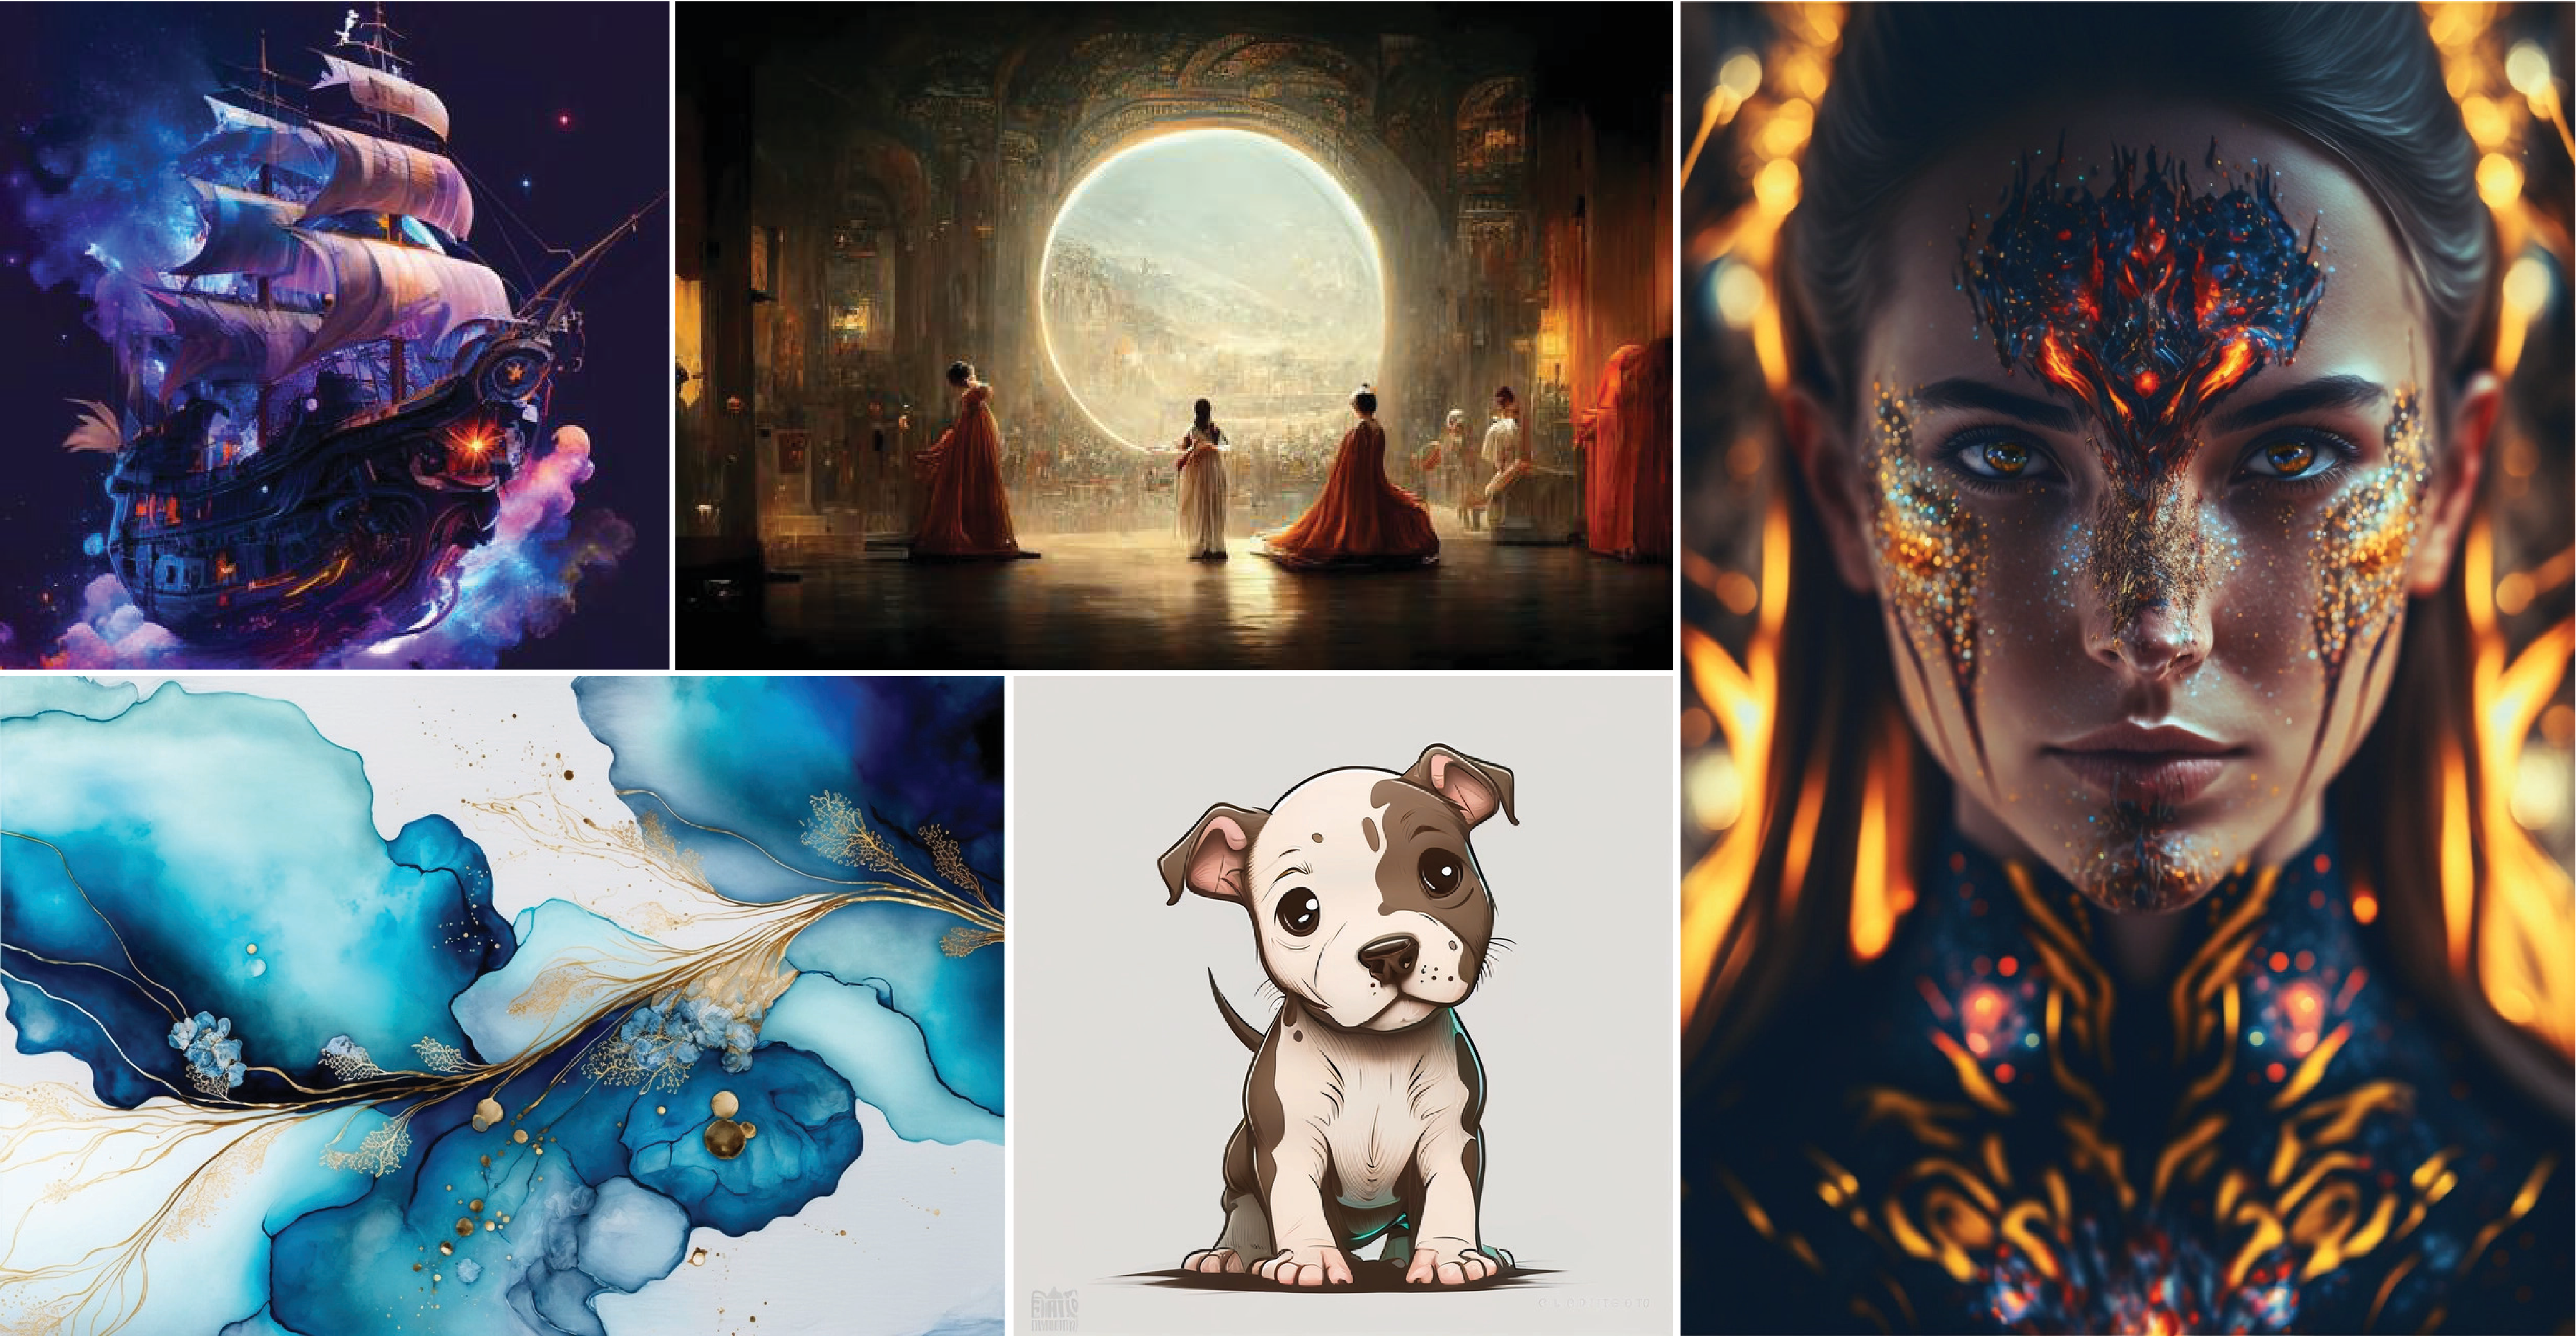
\includegraphics[width=1\columnwidth]{plots/overview/ai-art.pdf}
  \vspace{-0.25in}
  \caption{Sample AI-generated art pieces from the Midjourney
    community showcase \cite{mid-top-artistname,winaward}. }
  \label{fig:aiart}
\end{figure}

Today, all of these consequences have indeed occurred in the span of a few
months. Art students are quitting the field; AI models that mimic specific
artists are uploaded and shared for free; and professional artists are losing
their livelihoods to models mimicking their unique styles. Artists are
fighting back via lawsuits~\cite{ailawsuit,class-action}, online boycotts and
petitions~\cite{aiprotest}, but legal and regulatory action can take years,
and are difficult to enforce internationally. Thus most artists are faced a
choice to 1) do nothing, or 2) stop sharing samples of their art online to
avoid training models, and in doing so cripple their main way to advertise
and promote their work to customers.

In this paper, we present the design, implementation and evaluation of a
technical alternative to protect artists against style mimicry by
text-to-image diffusion models. 
We present Glaze, a system that allows an artist to apply carefully
computed perturbations to their art, such that diffusion models will learn
significantly altered versions of their style, and be ineffective in future
attempts at style mimicry. We worked closely with members of the professional
artist community to develop Glaze, and conduct multiple user studies with
1,156 participants from the artist community to evaluate its efficacy,
usability, and robustness against a variety of active countermeasures.

Intuitively, \system{} works by taking a piece of artwork, and computing a
minimal perturbation (a ``style cloak'') which, when applied, shifts the artwork's
representation in the generator model's feature space towards a chosen target
art style. Training on multiple cloaked images teaches the generator model
to shift the artistic style it associates with the artist, leading to mimicry
art that fails to match the artist's true style.

{Our work makes several key contributions:}
\vspace{-0.1in}
\begin{packed_itemize}
\item We engage with top professional artists and the broader community, and
  conduct user studies to understand their views and concerns towards AI art
  and the impact on their careers and community.
\item We propose \system{}, a system that protects artists from style mimicry
  by adding minimal perturbations to their artwork to mislead AI models to
  generate art different from the targeted artist. 92\% of surveyed artists
  find the perturbations small enough not to disrupt the value of their art. 
\item Surveyed artists find that \system{} successfully disrupts
  style mimicry by AI models on protected artwork. 93\% of 
  artists rate the protection is successful under a variety of settings,
  including tests against real-world mimicry platforms.
\item In challenging scenarios where an artist has already posted significant
  artworks online, we show \system{} protection remains high. 87.2\% of
  surveyed artists rate the protection as successful when an artist is only
  able to cloak 1/4 of their online art (75\% of art is uncloaked).
\item We evaluate \system{} and show that it is robust (protection success
  > 85\%) to a variety of adaptive countermeasures.
\item We discuss \system{} deployment and post-deployment
  experiences, including countermeasures in the wild.  
\end{packed_itemize}

\para{Ethics.} Our user study was reviewed and approved by our institutional
review board (IRB). All art samples used in experiments were used with
explicit consent by their respective artists. All user study participants
were compensated for their time, although many refused payment. 
